\begin{appendix} 

\renewcommand\section{\stdsection}

\newpage

\section*{Anhang} 
\addcontentsline{toc}{section}{Anhang}%\addtocontents{toc}{\vfill}
\renewcommand{\thesubsection}{\Alph{subsection}}

\subsection{Screenshots von QlikView} 
\label{lab:ScreenshotsVonQlikView}

\begin{figure}[htbp]
	\centering
		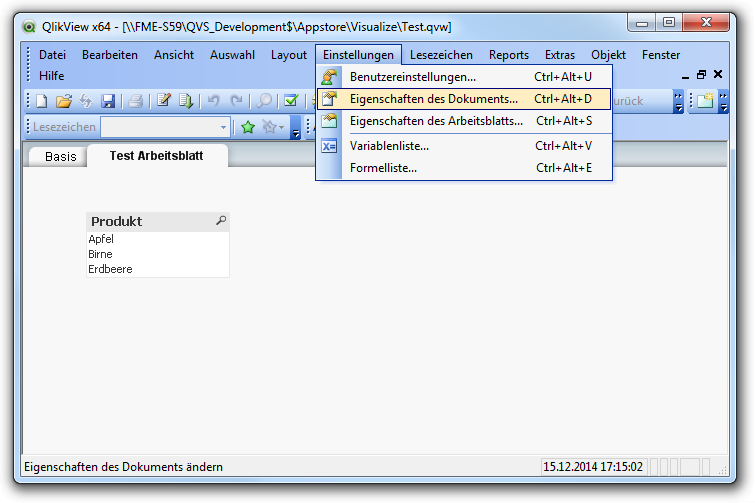
\includegraphics[width=1.00\textwidth]{img/DocumentExtensionListe/EigenschaftendesDokumentes.png}
	\caption[Öffnen der Eigenschaften des Dokumentes in QlikView]{Öffnen der Eigenschaften des Dokumentes in QlikView, \\Quelle: Eigene Abbildung}
	\label{fig:EigenschaftendesDokumentes}
\end{figure}


\begin{figure}[htbp]
	\centering
		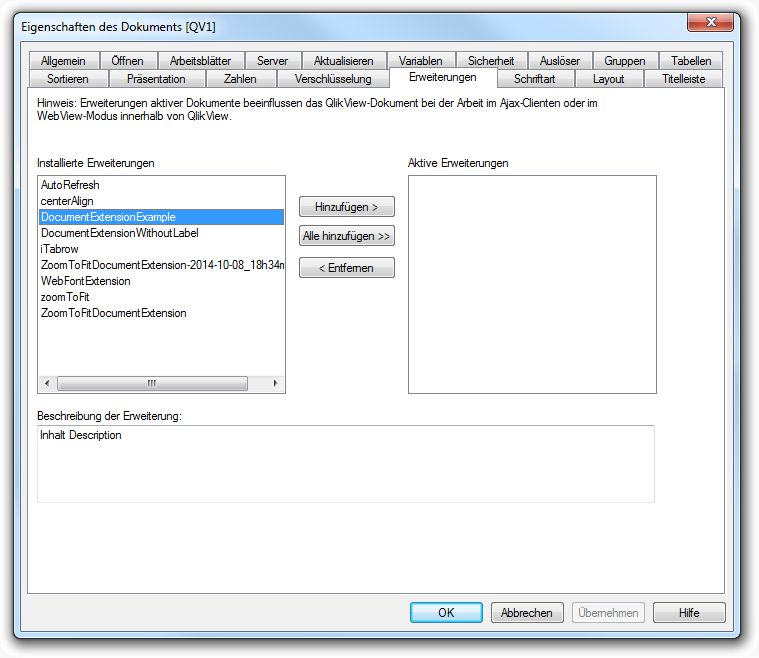
\includegraphics[width=1.00\textwidth]{./img/DocumentExtensionListe/DocumentExtensionListe.png}
	\caption[Liste der verfügbaren Document Extensions]{Liste der verfügbaren Document Extensions zum Hinzufügen zum QlikView-Dokument, Quelle: Eigene Abbildung}
	\label{fig:DocumentExtensionListe}
\end{figure}
% Beispiel Dateien erstellen
% Aus aktuellem Beispiel die Platzhalter rausnehmen




\begin{figure}[htbp]
	\centering
		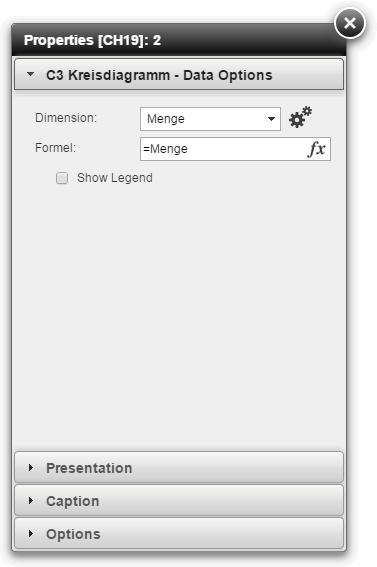
\includegraphics[width=0.70\textwidth]{img/QvPropDialog/C3KreisdiagrammDialog.png}
	\caption[QlikView JavaScript C3 Kreisdiagramm Konfigurationsdialog]{Screenshot des QlikView JavaScript C3 Kreisdiagramm Konfigurationsdialoges, Quelle: Eigene Abbildung}
	\label{fig:QlikViewC3KreisdiagrammDialogScreenshot}
\end{figure}




\begin{figure}[htbp]
	\centering
		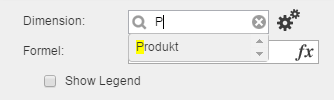
\includegraphics[width=0.60\textwidth]{img/QvPropDialog/DimensionAutomatischeVervollstaendigung.png}
		\caption[Automatischen Vervollständigung der Dimension]{Screenshot der automatischen Vervollständigung der Dimension, \\Quelle: Eigene Abbildung}
	\label{fig:DimensionAutomatischeVervollstaendigung}
\end{figure}



\begin{figure}[htbp]
	\centering
		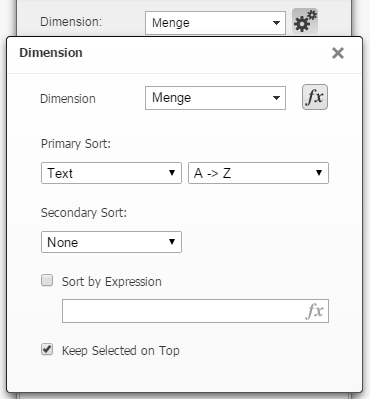
\includegraphics[width=0.70\textwidth]{img/QvPropDialog/DimensionSortierung.png}
	\caption[QlikView JavaScript C3 Kreisdiagramm Sortierungskonfiguration]{QlikView JavaScript C3 Kreisdiagramm Sortierungskonfiguration, \\Quelle: Eigene Abbildung}
	\label{fig:DimensionSortierung}
\end{figure}

\newpage
\subsection{Properties.qvpp-Datei des C3Kreisdiagramm Extension Objects} 
\label{lab:QlikViewJavascriptC3KreisdiagrammKonfigurationsdialog} 

\begin{listing}[htbp]
\begin{minted}[mathescape,
               linenos,
               numbersep=5pt,
							fontsize=\small,
               gobble=0,
               frame=lines,
							 fontsize=\scriptsize,
               framesep=2mm]{html}
<div class="ToolWindow-MainBody" avq="foldOutMenu:."
  style="overflow: visible !important; float: left;">
  <div class="prop-accordion" avq="accordion:.">
    <h3 class="prop-h3 accordion-shadow">
      <a href="#"> C3 Kreisdiagramm - Data Options </a>
    </h3>
    <div class="prop-grid_container accordion-shadow-enabler"
      style="overflow:auto;">
      <div class="prop-grid_clear 
        prop-grid_top-vertical-spacer-12px prop-grid_last"></div>
      <div class='prop-grid_clear prop-grid_prepend-1 prop-grid_span-5'
        avq='prop_label'>Dimension:</div>
      <div class='prop-grid_span-10 prop-grid_last'>
        <div class='prop-grid_span-7' 
          avq='prop_dynamicDropdown:.Chart.Dimension.0.Field'></div>
        <div class='prop-width-28px' propicontype='tool'
          avq='prop_dlgbuttonjqui:.Chart.Dimension.0:ExtensionDimDialog.qvpp'>
        </div>
      </div><br />
      <div class='prop-grid_clear prop-grid_prepend-1 prop-grid_span-5'
        avq='prop_label'>Formel:</div>
      <div class='prop-grid_span-10 prop-grid_last'>
        <div class='prop-grid_span-7 prop-grid_last'
          style='width:94%;' 
          avq='prop_editexpression:.Chart.Expression.0.0.Definition'></div>
      </div><br />
      <div class='prop-grid_clear prop-grid_prepend-1'>
        <div class='prop-grid_span-1'></div>
        <div class='prop-grid_span-1' 
          avq='prop_checkbox:.Chart.Text.0.Content'></div>
        <div class='prop-grid_span-7 prop-grid_last'
          avq='prop_label'>Zeige Legende:</div>
      </div>
    </div>
    <h3 class="prop-h3 accordion-shadow" avq="activeAccordionHeader:.:GenericPresentationFoldout.qvpp">
      <a href="#">Presentation</a></h3>
    <div class="prop-grid_container accordion-shadow-enabler" style="height:300px;"
      avq="panel::Layout.qvpp"></div>
    <h3 class="prop-h3 accordion-shadow" avq="activeAccordionHeader::PropertiesCaptionFoldout.qvpp">
      <a href="#">Caption</a></h3>
    <div class="prop-grid_container accordion-shadow-enabler" avq="panel::Caption.qvpp"></div>
      <h3 class="prop-h3 accordion-shadow" avq="activeAccordionHeader:.:PropertiesOptionsFoldout.qvpp">
      <a href="#">Options</a></h3>
    <div class="prop-grid_container accordion-shadow-enabler" avq="panel::Options.qvpp"></div>
  </div><span class="bottom-gap"></span>
</div>
\end{minted}
\caption[\textit{Properties.qvpp}-Datei des QlikView C3Kreisdiagramm Extension Objects]{\textit{Properties.qvpp}-Datei des QlikView C3Kreisdiagramm Extension Objects, Quellcode\textbackslash{}JavaScript\textbackslash{}QlikView\textbackslash{}C3Kreisdiagramm\textbackslash{}Properties.qvpp, \\Quelle: Eigenes Listing}
\label{lst:QlikViewJavascriptC3KreisdiagrammSkript}
\end{listing}

\newpage
\subsection{Screenshots von Qlik Sense} 
\label{lab:ScreenshotsVonQlikSense} 

\begin{figure}[htbp]
	\centering
		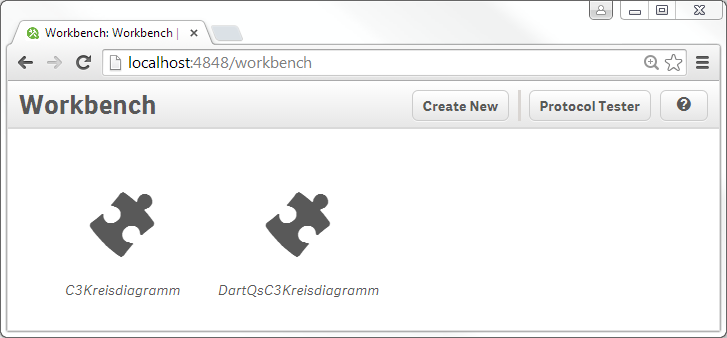
\includegraphics[width=1.00\textwidth]{img/SenseScreenshots/Workbench.PNG}
	\caption[Screenshot der Qlik Sense Workbench]{Screenshot der Qlik Sense Workbench, Quelle: Eigene Abbildung}
	\label{fig:Workbench}
\end{figure}

\begin{figure}[htbp]
	\centering
		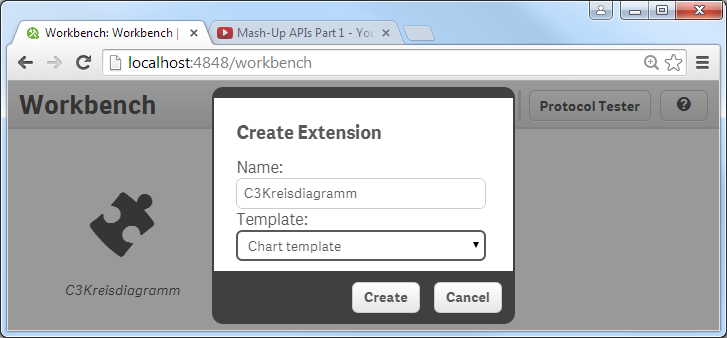
\includegraphics[width=1.00\textwidth]{img/SenseScreenshots/WorkbenchCreateNew.PNG}
	\caption[Screenshot des Dialoges zur Erstellung eines Qlik Sense Extension Objects]{Screenshot des Dialoges zur Erstellung eines Qlik Sense Extension Objects, \\Quelle: Eigene Abbildung}
	\label{fig:WorkbenchCreateNew}
\end{figure}

\newpage

\begin{figure}[htbp]
	\centering
		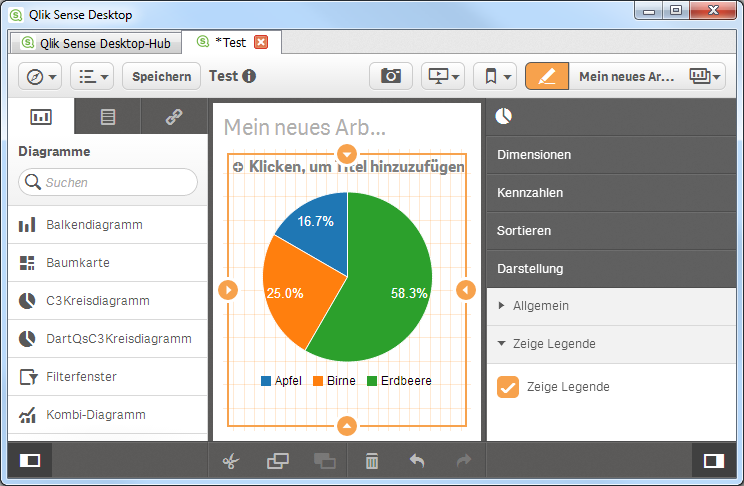
\includegraphics[width=1.00\textwidth]{img/SenseScreenshots/ArbeitsblattQlikSense.PNG}
	\caption[Screenshot des C3Kreisdiagramms in einem Qlik Sense Arbeitsblatt]{Screenshot eines Qlik Sense Arbeitsblattes mit der hinzugefügten Erweiterung C3Kreisdiagramm - mitte - und eingeblendetem \textit{accordion} zur Konfiguration - rechts, Quelle: Eigene Abbildung}
	\label{fig:ArbeitsblattQlikSense}
\end{figure}


\newpage
\subsection{Beispiel-Screenshot der DownloadArbeitsblattAlsPng-Erweiterung} 
\label{lab:BeispielScreenshotDownloadArbeitsblattAlsPng} 



\begin{figure}[htbp]
	\centering
		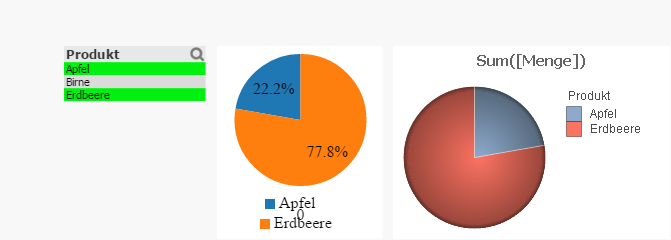
\includegraphics[width=1.00\textwidth]{img/ScreenshotSheet/ScreenshotSheet.png}
	\caption[Durch die Erweiterung DownloadArbeitsblattAlsPng heruntergeladener Screenshot]{Durch die Erweiterung DownloadArbeitsblattAlsPng heruntergeladener Screenshot, \\Quelle: Eigene Abbildung}
	\label{fig:ScreenshotSheet}
\end{figure}


\newpage
\subsection{initialProperties für ein Qlik Sense Extension Object in Dart-Syntax} 
\label{lab:initialPropertiesQlikSenseExtensionObjectDartSyntax} 

Im Listing \ref{lst:initialPropertiesQlikSenseExtensionObjectDartSyntax} ist die testweise Portierung der \textit{initialProperties.js}-Datei zu sehen. In den Zeilen 4, 5 und 6 ist die Erstellung von JavaScript-Proxy-Objekten mithilfe des Konstruktors \textit{JsObject.jsify} zu sehen. Dies es notwendig, denn in Dart erstellte Kollektionen sind nicht mit JavaScript kompatibel, auch wenn es sich um leere Listen wie in den Zeilen 4 und 5 handelt. Daher müssen sie konvertiert werden.

\begin{listing}[htbp]
\begin{minted}[mathescape,
               linenos,
               numbersep=5pt,
               gobble=0,
               frame=lines,
							fontsize=\footnotesize,
               framesep=2mm]{html}
'initialProperties': {
  'version': 1.0,
  'qHyperCubeDef': {
    'qDimensions': new JsObject.jsify([]),
    'qMeasures': new JsObject.jsify([]),
    'qInitialDataFetch': new JsObject.jsify([{
      'qWidth': 10,
      'qHeight': 50
    }])
  }
}
\end{minted}
\caption[\textit{initialProperties} für ein Qlik Sense Extension Object in Dart-Syntax]{\textit{initialProperties} für ein Qlik Sense Extension Object in Dart-Syntax, \\Quelle: Eigenes Listing}
\label{lst:initialPropertiesQlikSenseExtensionObjectDartSyntax}
\end{listing}


\newpage
\subsection{Klassendiagramm des Projektes qlikview""\_qlik""\_sense""\_extensions} 
\label{lab:KlassendiagrammDerKlassenbibliothek} 

\begin{figure}[htbp]
	\centering
		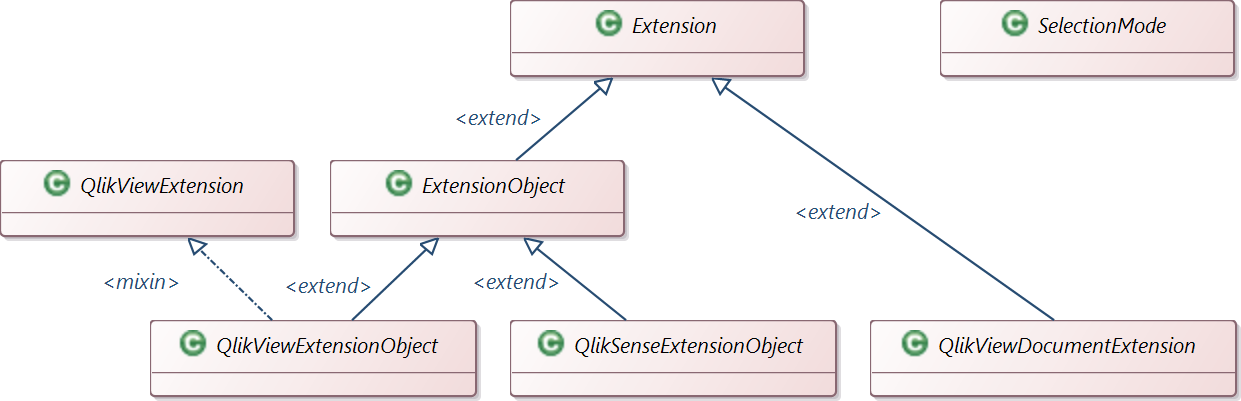
\includegraphics[width=1.00\textwidth]{img/Klassendiagramm/Klassendiagramm.png}
	\caption[Klassendiagramm der Klassenbibliothek \textit{qlikview\_qlik\_sense\_extensions}]{Klassendiagramm der Klassenbibliothek \textit{qlikview\_qlik\_sense\_extensions}, Quelle: Eigene Abbildung}
	\label{fig:Klassendiagramm}
\end{figure}


\newpage
\subsection{Listings zu source maps} 
\label{lab:ListingsZuSourceMaps} 

\begin{listing}[htbp]
\begin{minted}[mathescape,
               linenos,
               numbersep=5pt,
               gobble=0,
               frame=lines,
							fontsize=\footnotesize,
               framesep=2mm]{Bash}
# sourceMappingURL=main.dart.js.map
\end{minted}
\caption[Beispiel für einen Verweis auf eine source map]{Beispiel für einen Verweis auf eine source map, Quelle: Eigenes Listing}
\label{lst:BeispielVerweisSourceMap}
\end{listing}

\begin{listing}[htbp]
\begin{minted}[mathescape,
               linenos,
               numbersep=5pt,
               gobble=0,
               frame=lines,
							fontsize=\scriptsize,
               framesep=2mm]{javascript}
{
  "version": 3,
  "file": "main.dart.js",
  "sourceRoot": "",
  "sources": ["packages/$sdk/lib/_internal/compiler/js_lib/interceptors.dart" 
             ,"packages/$sdk/lib/_internal/compiler/js_lib/js_array.dart" 
             ,"packages/$sdk/lib/collection/list.dart" 
             ,"packages/$sdk/lib/internal/iterable.dart" 
             ,"packages/$sdk/lib/_internal/compiler/js_lib/js_number.dart" 
             ,"packages/$sdk/lib/_internal/compiler/js_lib/js_string.dart" 
             ,"packages/$sdk/lib/_internal/compiler/js_lib/isolate_helper.dart" 
             ,"packages/$sdk/lib/collection/queue.dart" 
             ,"packages/$sdk/lib/_internal/compiler/js_lib/js_helper.dart" 
             ,"packages/$sdk/lib/_internal/compiler/js_lib/collection_patch.dart" 
             ,"packages/$sdk/lib/collection/iterable.dart" 
             ,"packages/$sdk/lib/async/timer.dart" 
             ,"packages/$sdk/lib/_internal/compiler/js_lib/native_helper.dart" 
             ,"packages/$sdk/lib/_internal/compiler/js_lib/js_rti.dart" 
             ,"packages/$sdk/lib/internal/lists.dart" 
             ,"packages/$sdk/lib/internal/symbol.dart" 
             ,"packages/$sdk/lib/_internal/compiler/js_lib/js_names.dart" 
             ,"packages/$sdk/lib/_internal/compiler/js_lib/async_patch.dart" 
             ,"packages/$sdk/lib/async/async_error.dart" 
             ,"packages/$sdk/lib/async/future.dart" 
             ,"packages/$sdk/lib/async/future_impl.dart" 
             ,"packages/$sdk/lib/async/schedule_microtask.dart" 
             ,"packages/$sdk/lib/async/zone.dart" 
             ,"packages/$sdk/lib/core/duration.dart" 
             ,"packages/$sdk/lib/collection/hash_map.dart" 
             ,"packages/$sdk/lib/_internal/compiler/js_lib/core_patch.dart" 
             ,"packages/$sdk/lib/collection/maps.dart" 
             ,"packages/$sdk/lib/collection/set.dart" 
             ,"packages/$sdk/lib/core/errors.dart" 
             ,"packages/$sdk/lib/core/exceptions.dart" 
             ,"packages/$sdk/lib/core/print.dart" 
             ,"packages/$sdk/lib/_internal/compiler/js_lib/internal_patch.dart" 
             ,"packages/$sdk/lib/core/expando.dart" 
             ,"packages/$sdk/lib/core/null.dart" 
             ,"packages/$sdk/lib/core/object.dart" 
             ,"packages/$sdk/lib/core/string_buffer.dart" 
             ,"packages/$sdk/lib/html/dart2js/html_dart2js.dart" 
             ,"packages/$sdk/lib/_internal/compiler/js_lib/native_typed_data.dart" 
             ,"packages/$sdk/lib/_internal/compiler/js_lib/js_primitives.dart" 
             ,"main.dart"],
\end{minted}
\caption[Auszug einer formatierten source map]{Auszug einer formatierten source map, Quelle: Eigenes Listing}
\label{lst:AuszugEinerFormatiertenSourceMap}
\end{listing}


\newpage
\subsection{Fehlerhafte Verwendung der QlikView Ajax API} 
\label{lab:FehlerhafteVerwendungDerQlikViewAjaxAPI} 

Im Listing \ref{lst:AnimatedScatterChartScriptJsDatei} ist ein Auszug aus der \textit{Script.js}-Datei der QlikView Extension \textit{Animated Scatter Chart} zu sehen. In der Zeile 3 wird der Funktion \textit{AddExtension} die Callback-Funktion übergeben, welche unter anderem auch den Aufruf der Funktionen \textit{LoadCSS} in Zeile 30 und \textit{LoadExtensionScripts} in Zeile 37 enthält. Doch da die Callback-Funktion bei jedem Zeichnen aufgerufen wird, werden diese Ressourcen auch bei jedem Zeichnen erneut dem \textit{head}-Element des Dokuments hinzugefügt.

\begin{listing}[htbp]
\begin{minted}[mathescape,
               linenos,
               numbersep=5pt,
							fontsize=\footnotesize,
               gobble=0,
               frame=lines,
               framesep=2mm]{javascript}
function D3AnimatedScatterChart_Init() {

    Qva.AddExtension("D3AnimatedScatterChart",
        function() {

          ConsoleClear();
          fixSelectBox();

          var _this = this;
          _this.ExtSettings = {};
          _this.ExtSettings.ExtensionName = 'D3AnimatedScatterChart';
          _this.ExtData = {};

          // Base Url for CSS Files
          _this.ExtSettings.LoadUrl = Qva.Remote + (Qva.Remote.indexOf('?') >=
            0 ? '&' : '?') + 'public=only' + '&name=';

          //Todo: Can be removed in final version
          _this.ExtSettings.DataFile = Qva.Remote + (Qva.Remote.indexOf('?') >=
              0 ? '&' : '?') + 'public=only' +
            '&name=Extensions/D3AnimatedScatterChart/lib/data/nations.json';
          _this.ExtSettings.DataFile_Full = Qva.Remote + (Qva.Remote.indexOf(
              '?') >= 0 ? '&' : '?') + 'public=only' +
            '&name=Extensions/D3AnimatedScatterChart/lib/data/nations_full.json';

          var cssFiles = [];
          cssFiles.push('Extensions/' + _this.ExtSettings.ExtensionName +
            '/lib/css/style.css');
          for (var i = 0; i < cssFiles.length; i++) {
            Qva.LoadCSS(_this.ExtSettings.LoadUrl + cssFiles[i]);
          }

          var jsFiles = [];
          //http://d3js.org/d3.v2.js?2.8.1
          jsFiles.push('Extensions/' + _this.ExtSettings.ExtensionName +
            '/lib/js/d3_v2.js');
          Qv.LoadExtensionScripts(jsFiles, function() {
\end{minted}
\caption[Formatierter Auszug der \textit{Script.js}-Datei des Animated Scatter Chart]{Formatierter Auszug der \textit{Script.js}-Datei des Animated Scatter Chart, \\Quelle: \cite{QlikViewExtensionAnimatedScatterChartSourceCode}}
\label{lst:AnimatedScatterChartScriptJsDatei}
\end{listing}

Die Abbildung \ref{fig:endOfHead} zeigt, dass diese Ressourcen tatsächlich mehrfach im \textit{head}-element des Dokuments auftauchen. In Abbildung \ref{fig:Sources} ist darüber hinaus zu sehen, dass diese Dateien bei deaktiviertem Browsercache sogar mehrfach vom Server angefragt und erneut heruntergeladen werden.

\begin{figure}[htbp]
	\centering
		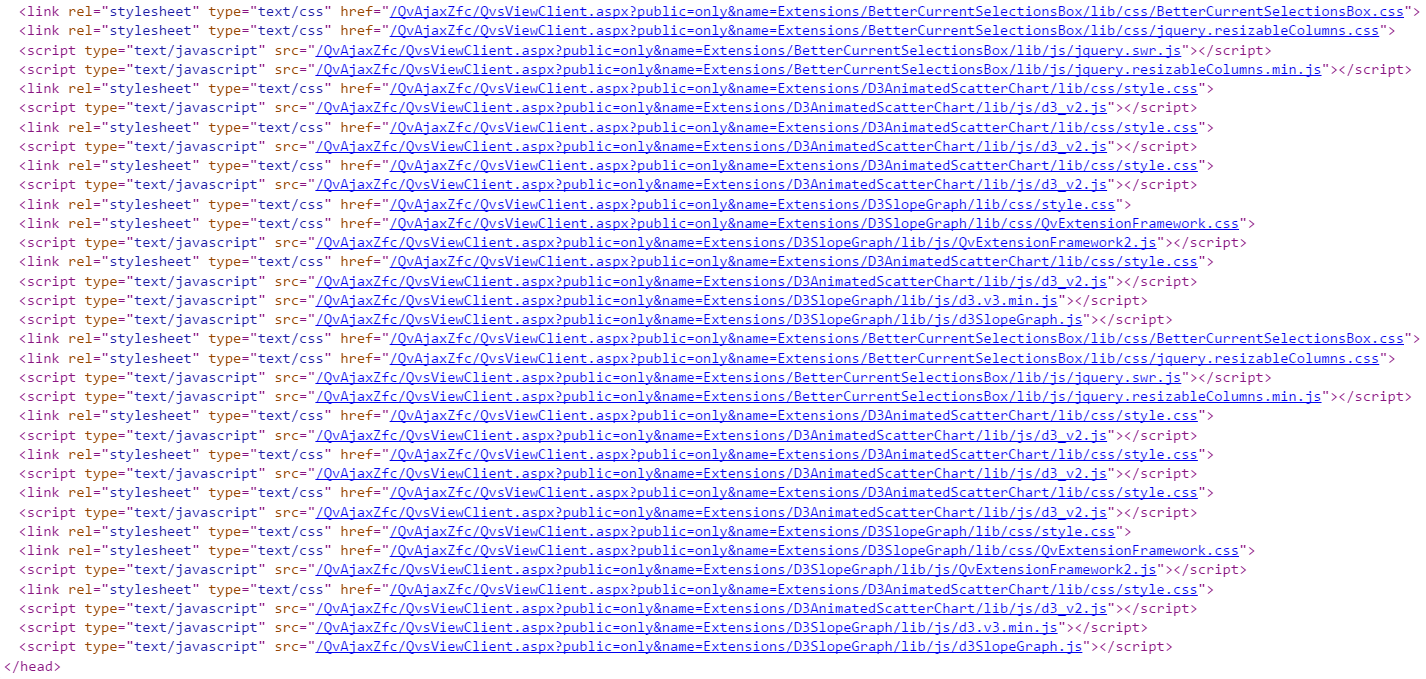
\includegraphics[width=1.00\textwidth]{img/headRudundant/endOfHead.PNG}
	\caption[Redundante Einträge im \textit{head}-Element des Dokuments]{Durch fehlerhafte Verwendung der QlikView Ajax API tauchen redundante Einträge im \textit{head}-Element des Dokuments auf, \\Quelle: Eigene Abbildung}
	\label{fig:endOfHead}
\end{figure}

\begin{figure}[htbp]
	\centering
		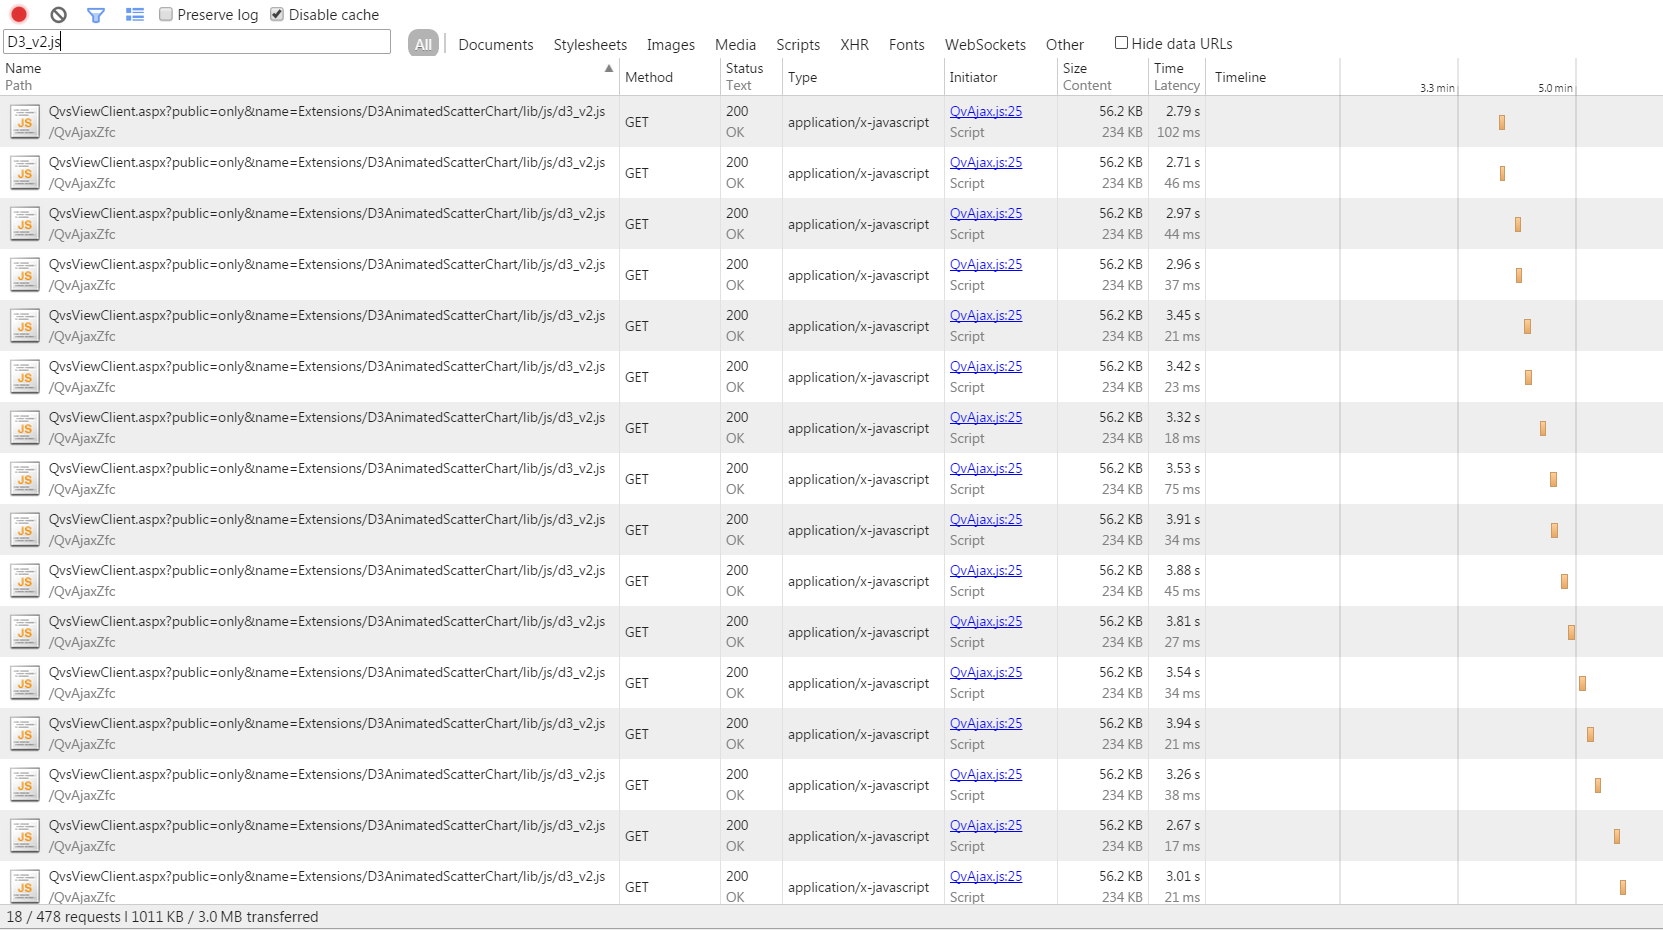
\includegraphics[width=1.00\textwidth]{img/headRudundant/Sources.png}
	\caption[Mehrfaches Herunterladen derselben Datei.]{Die Filterung nach der Bibliothek d3\_v2 zeigt, dass bei deaktiviertem Browsercache dieselbe Datei mehrfach heruntergeladen wird, \\Quelle: Eigene Abbildung}
	\label{fig:Sources}
\end{figure}


\newpage
\subsection{Abbildungen zur erleichterten Entwicklung mit Dart} 
\label{lab:AbbildungenZurErleichtertenEntwicklungVonErweiterungenMitDart}

Mit einem Rechtsklick im Editor öffnet sich ein Kontextmenü, in dem unter anderem der Eintrag \textit{Quick Fix} verfügbar ist. Alternativ kann die Funktion mit der Tastenkombination Steuerung + 1 aufgerufen werden. Bei Fehlermeldungen und Warnungen bietet sie Lösungsvorschläge an und generiert automatisch den passenden Code.

\begin{figure}[htbp]
	\centering
		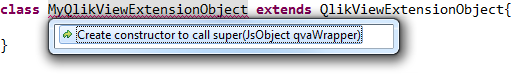
\includegraphics[width=1.00\textwidth]{img/HilfeDurchEditor/implConstr.png}
	\caption[Vorschlag zur automatischen Implementierung des Konstruktors]{Vorschlag zur automatischen Implementierung des Konstruktors, \\Quelle: Eigene Abbildung}
	\label{fig:implConstr}
\end{figure}

In Abbildung \ref{fig:implConstr} ist zu sehen, dass der Klasse \textit{MyQlikViewExtensionObject} der Aufruf des Konstruktors der Basisklasse fehlt. Die automatische Implementierung des Konstruktors wird angeboten. Anschließend wird eine Warnung ausgegeben, dass zwei Schnittstellen in der konkreten Klasse noch immer nicht implementiert sind.

\begin{figure}[htbp]
	\centering
		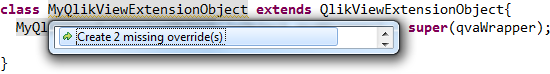
\includegraphics[width=1.00\textwidth]{img/HilfeDurchEditor/implOverride.png}
	\caption[Vorschlag zur automatischen Implementierung der fehlenden Schnittstellen]{Vorschlag zur automatischen Implementierung der fehlenden Schnittstellen, \\Quelle: Eigene Abbildung}
	\label{fig:implOverride}
\end{figure}

Abbildung \ref{fig:implOverride} zeigt, dass in diesem Fall die Generierung der Methodenköpfe angeboten wird. Die vollständige Struktur der Klasse ist in Abbildung \ref{fig:complete} zu sehen. Nach dem Eingeben von \textit{this.} erscheint eine Liste von Vorschlägen für automatische Vervollständigungen. In der Liste sind lediglich die im Kontext sichtbaren Felder und Methoden aufgeführt. Diese Hilfestellungen erleichtern die Einarbeitung, beschleunigen die Entwicklung und beugen Fehlern vor.

\begin{figure}[htbp]
	\centering
		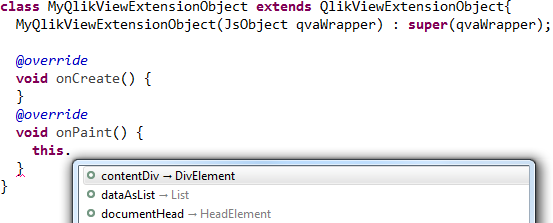
\includegraphics[width=1.00\textwidth]{img/HilfeDurchEditor/complete.png}
	\caption[Automatische Vervollständigung der möglichen Felder und Methoden]{Automatische Vervollständigung der möglichen Felder und Methoden, Quelle: Eigene Abbildung}
	\label{fig:complete}
\end{figure}



\end{appendix} 
